\documentclass[a4paper]{article}

\title{PH2255 Course:\\
Introduction to Statistical Methods\\Exercise 1}
\author{Thomas Bass}
\date{15 January 2021}

% LaTeX preambule: loading relevant packages, configuring Python listings
\usepackage{graphicx}
\usepackage{amsmath}
\usepackage{color}
\usepackage{listings}
\usepackage{hyperref}
\usepackage{bm}

\definecolor{dkgreen}{rgb}{0,0.6,0}
\definecolor{gray}{rgb}{0.5,0.5,0.5}
\definecolor{mauve}{rgb}{0.58,0,0.82}

% Settings for colour-coding and formatting Python code:
\lstset{
  language=Python,                % the language of the code
  basicstyle=\footnotesize,           % the size of the fonts that are used for the code
  numbers=left,                   % where to put the line-numbers
  numberstyle=\tiny\color{gray},  % the style that is used for the line-numbers
  stepnumber=5,                   % the step between two line-numbers. If it's 1, each line
                                  % will be numbered
  numbersep=5pt,                  % how far the line-numbers are from the code
  backgroundcolor=\color{white},      % choose the background color. You must add \usepackage{color}
  showspaces=false,               % show spaces adding particular underscores
  showstringspaces=false,         % underline spaces within strings
  showtabs=false,                 % show tabs within strings adding particular underscores
  frame=single,                   % adds a frame around the code
  rulecolor=\color{black},        % if not set, the frame-color may be changed on line-breaks within not-black text (e.g. commens (green here))
  tabsize=2,                      % sets default tabsize to 2 spaces
  captionpos=b,                   % sets the caption-position to bottom
  breaklines=true,                % sets automatic line breaking
  breakatwhitespace=false,        % sets if automatic breaks should only happen at whitespace
  title=\lstname,                   % show the filename of files included with \lstinputlisting;
                                  % also try caption instead of title
  keywordstyle=\color{blue},          % keyword style
  commentstyle=\color{dkgreen},       % comment style
  stringstyle=\color{mauve},         % string literal style
  escapeinside={\%*}{*)},            % if you want to add LaTeX within your code
  morekeywords={*,...}               % if you want to add more keywords to the set
}

\begin{document}
\maketitle

\begin{abstract}
Exercise One in the PH2255 course begins with an introduction to using the least-squares method provided in SciPy's \lstinline$curve_fit$ method, and using the error propagation formula described below to generate the standard deviation of the generated parameters. Plots are generated to show how well a least-squares method fits the data, using first, second, and third order polynomials.
\end{abstract}

First, we must ingest the data provided in the lab script into Python. We use Numpy's \lstinline$np.array$ as this will allow us to manipulate the data later.
\begin{lstlisting}
x = np.array([1.0, 2.0, 3.0, 4.0, 5.0, 6.0, 7.0, 8.0, 9.0])
y = np.array([2.7, 3.9, 5.5, 5.8, 6.5, 6.3, 7.7, 8.5, 8.7])
sig = np.array([0.3, 0.5, 0.7, 0.6, 0.4, 0.3, 0.7, 0.8, 0.5])
\end{lstlisting}
Now that the data is ingested, we can use SciPy's \lstinline$curve_fit$ method to generate the optimal values for the parameters, so that the sum of the squared residuals is minimized. 

First, we define a general polynomial function at a given value of \lstinline$x$ and list of coefficients \lstinline$theta$, using this general form of the polynomial function:
\begin{equation}
f(x) = \theta_0 + \theta_1 x + \theta_2x^2 + ...
\end{equation}
In python...
\begin{lstlisting}
def polynomial(x, *theta): 
	return sum([theta[i]*x**i for i in range(len(theta))])
\end{lstlisting}

This is a very efficient "one-liner" in python, using list comprehension to iterate over \lstinline$i$ for a range defined by the length of \lstinline$theta$. The use of \lstinline$*theta$ allows the parameter vector $\bm\theta = (\theta_0, \theta_1)$ to have arbitrary length, useful for coding higher order polynomials.

Next, we use the \lstinline$curve_fit$ to generate our parameters and covariance matrices for each of the first, second, and third order polynomials:
\begin{lstlisting}
p0_first = np.array([1.0, 1.0])
theta_hat_first, covariance_first = curve_fit(polynomial, x, y, p0_first, sig, absolute_sigma=True)
\end{lstlisting}

The same code was repeated, with renamed variables and corresponding \lstinline$p0$ arrays for the second and third order polynomials.

Now that we have the parameters, we can plot our fitted line using the corresponding parameters as polynomial coefficients. To do this in MatPlotLib, we define a function \lstinline$fit$, similar to \lstinline$polynomial$ but without the asterisk unpacking the array:
\begin{lstlisting}
def fit(x, theta): 
	return sum([theta[i]*x**i for i in range(len(theta)) ])
\end{lstlisting}

The exercise asks us to plot the standard deviation of the fitted function as well as the fit its self, so we use Equation 26 from the script (slightly modified for this specific use):
\begin{equation}
\sigma^2_f\approx\sum^m_{i,j=0}\frac{\partial f}{\partial\hat\theta_i}\frac{\partial f}{\partial\hat\theta_ij}U_{ij}
\end{equation}
Where $U_{ij} = \text{cov}[i, j]$. In our example, $f$ is the polynomial function, so the derivatives rapidly simplify with use of the Kronecker Delta function:
\begin{equation}
\frac{\partial f(x, \vec{\hat\theta})}{\partial\hat{\theta_i}} = \frac\partial{\partial\hat\theta_i}\sum^N_{k=0}\hat{\theta_k}x^k=\sum^N_{k=0}\delta_{ik}x^k=x^i
\end{equation}
This allows us to write the entire standard deviation formula very compactly:
\begin{equation}
\sigma^2_f=\sum^N_{i,j=0}x^{i+j}\text{cov}[i, j]
\end{equation}
In python...
\begin{lstlisting}
def std_dev(x, cov): 
	return sum([(x**(i+j))*cov[i][j] for i in range(len(cov)) for j in range(len(cov))])
\end{lstlisting}
This again uses compact list comprehension to iterate over \lstinline$i$ and \lstinline$j$, as defined by the length of the covariance matrix \lstinline$cov$. \emph{N.B.:} we take the square root of this function's results later, to reflect $\text{std. dev.}=\sqrt{\sigma^2}$.

We now use these two functions to plot our data in MatPlotLib (figure setup is omitted here):
\begin{lstlisting}
ax.errorbar(x, y, yerr=sig, fmt='kx', label="test data")
ax.plot(x_val, fit(x_val, theta_hat_first), 'r', label="first order fit")
ax.fill_between(x_val, fit(x_val, theta_hat_first)-np.sqrt(std_dev(x_val, covariance_first)), fit(x_val, theta_hat_first)+np.sqrt(std_dev(x_val, covariance_first)), label="one standard deviation")
\end{lstlisting}

This, generates the following plots for the first order fit, and modified and repeated code for the second and third order fits:
\begin{figure}[h]
\centerline{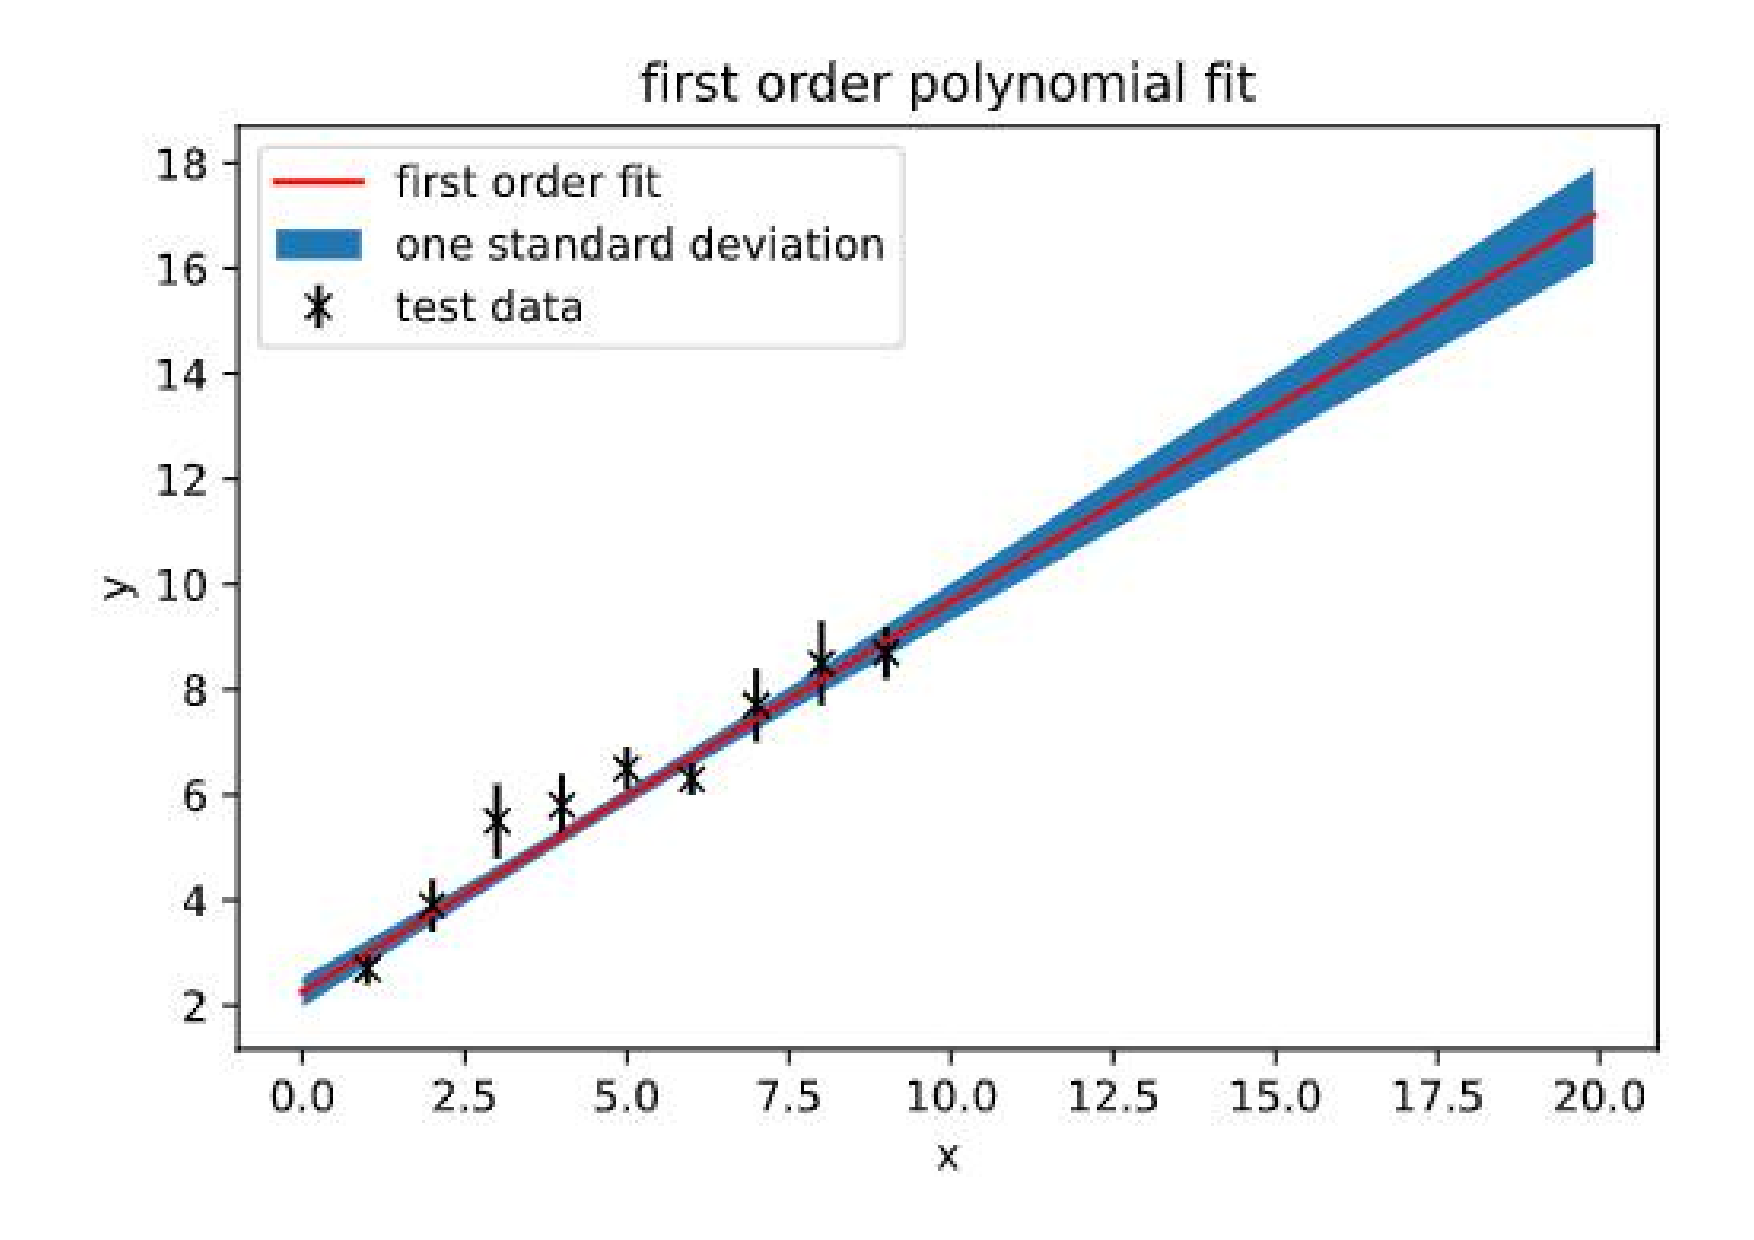
\includegraphics[scale=0.3]{first_order.pdf}}
\caption{First-order polynomial fit, showing fit curve and one standard deviation above and below}
\label{fig:firstorder}
\end{figure}

\begin{figure}[h]
\centerline{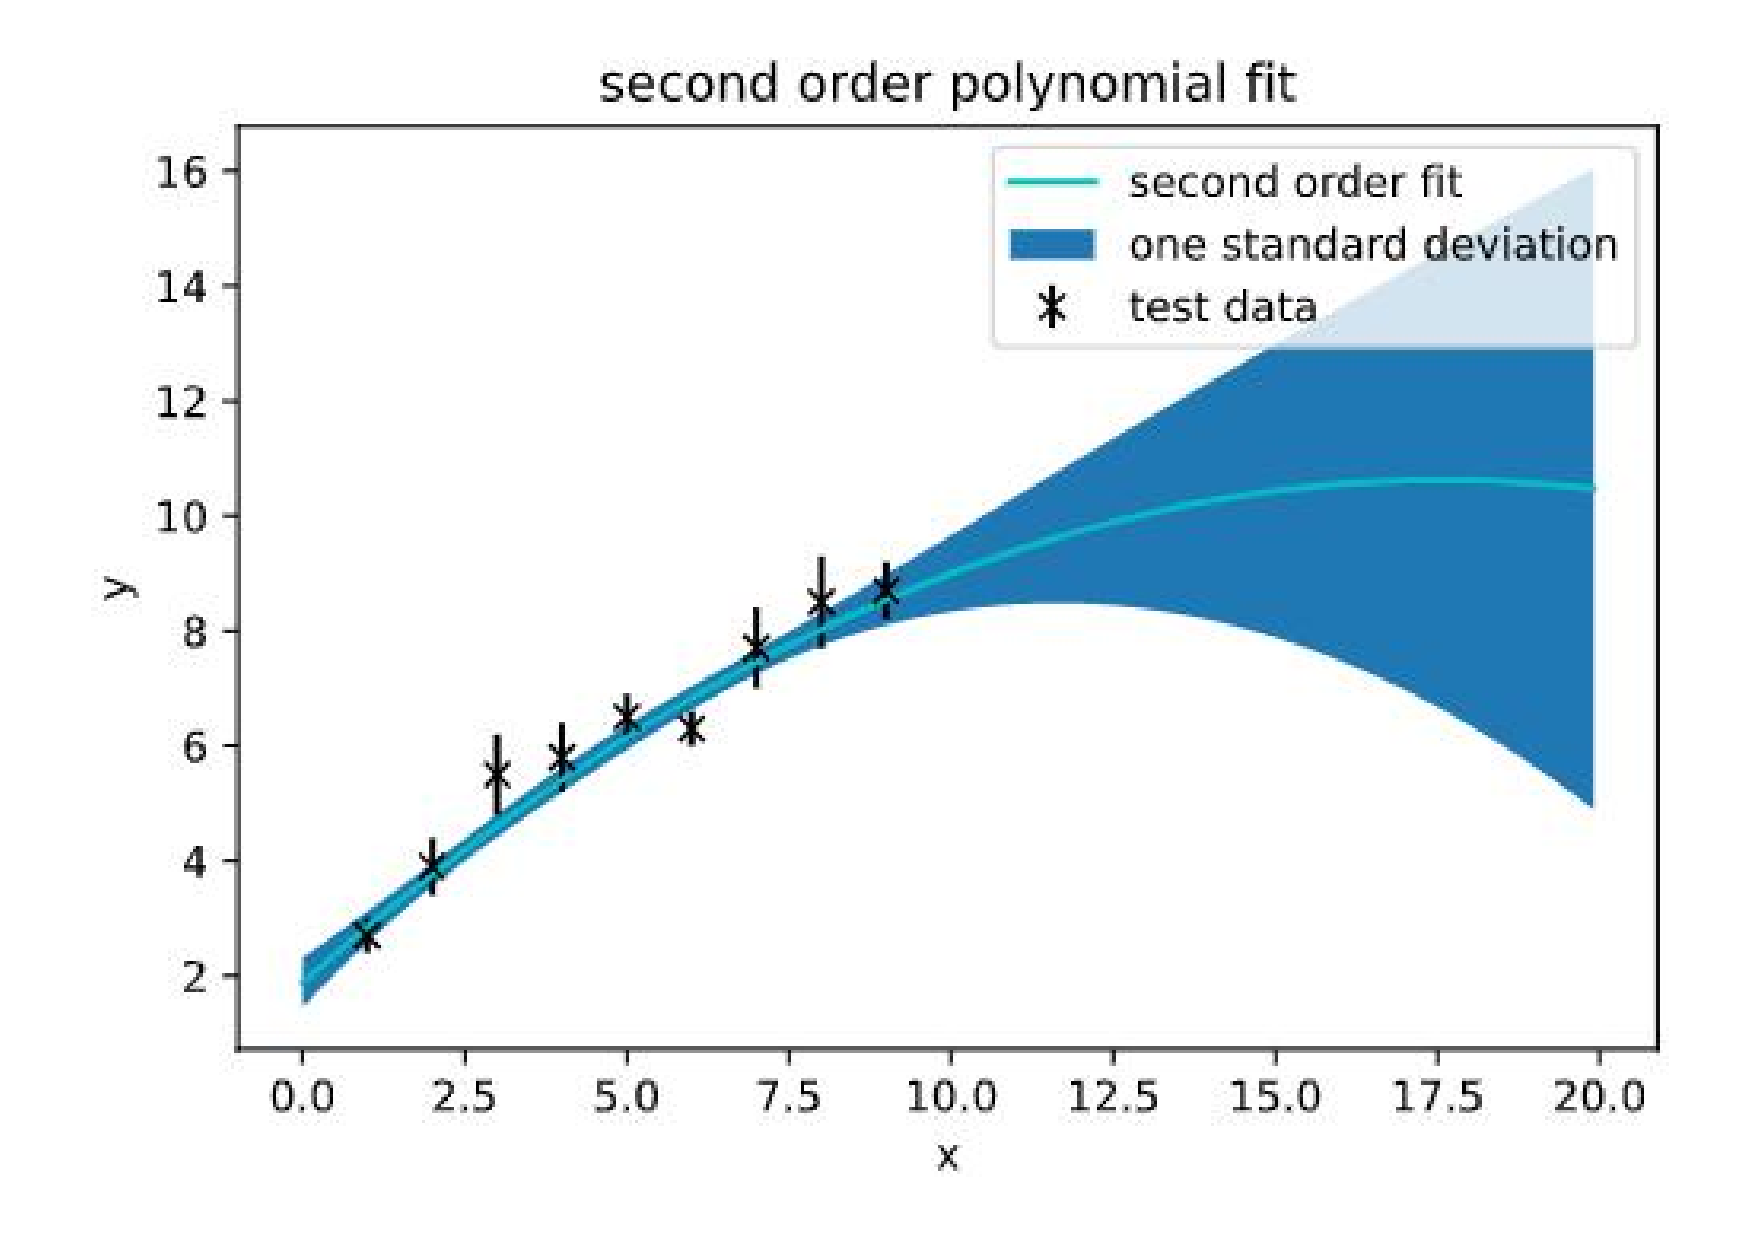
\includegraphics[scale=0.3]{second_order.pdf}}
\caption{Second-order polynomial fit, showing fit curve and one standard deviation above and below}
\label{fig:secondorder}
\end{figure}
\newpage
\begin{figure}[h!]
\centerline{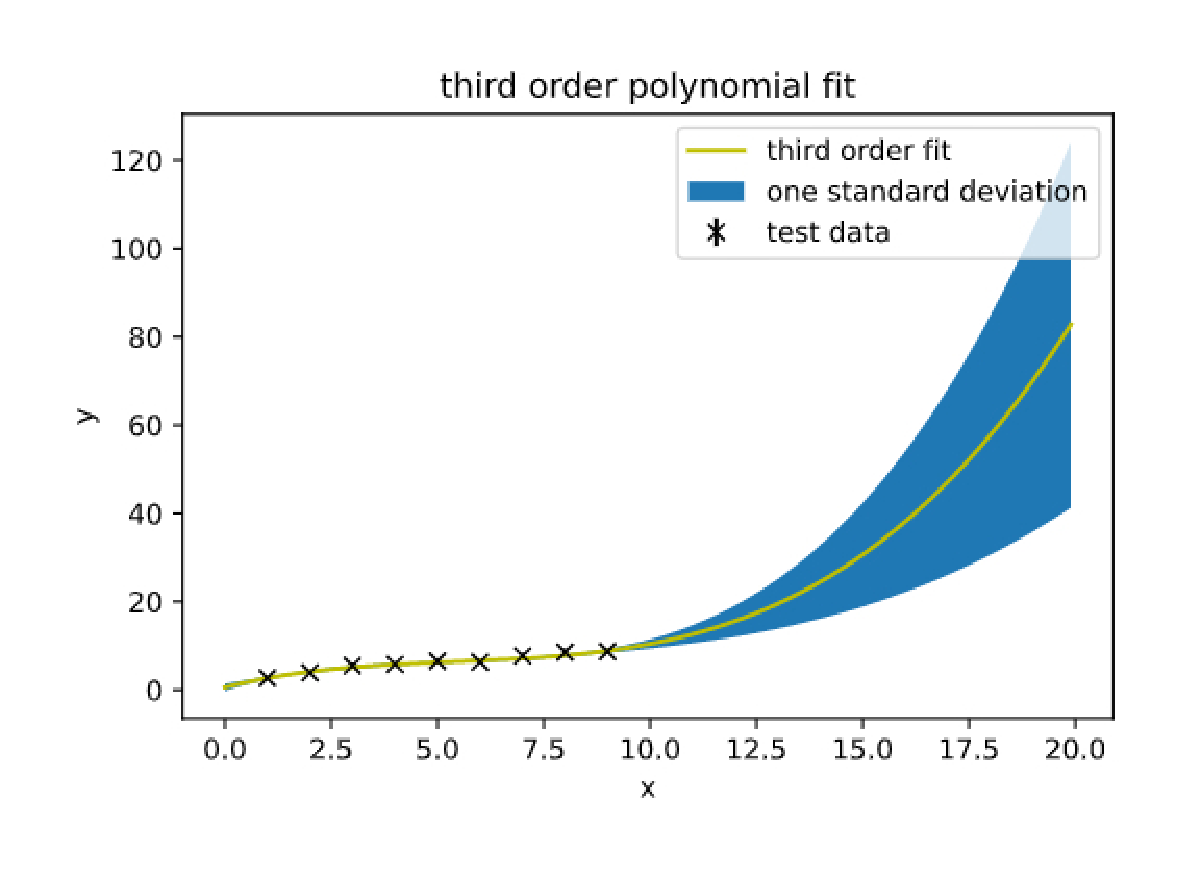
\includegraphics[scale=0.45]{third_order.pdf}}
\caption{Third-order polynomial fit, showing fit curve and one standard deviation above and below}
\label{fig:thirdorder}
\end{figure}
From these graphs, we can qualitatively see that the standard deviation for each fit extrapolated beyond the data sets increases more rapidly for higher-order polynomials.
\\\\
We can also generate chi-squared values for each of these fits, using the following code:
\begin{lstlisting}
sum(((y - polynomial(x, *theta_hat))/sig)**2)
\end{lstlisting}
The chi-squared values and degrees of freedom for each fit are tabulated below:
\begin{table}[h!]
\centering
\begin{tabular}{lll}
\hline
Polynomial Order & Chi-Squared       & Degrees of Freedom \\ \hline
1                & 8.2515361178354   & 7                  \\
2                & 6.842115296038535 & 6                  \\
3                & 3.747761582200386 & 5                  \\ \hline

\end{tabular}
\caption{\label{tab:chi-sq}Chi-square values and degrees of freedom for each fit.}
\end{table}
\newpage
\begin{appendix}
\section{Python Code}\label{sec:python}
The complete code used in this exercise is presented below, as well as the text outputs of the script:
\lstinputlisting[language=Python,frame=single]{py.py}%
\begin{lstlisting}
chisq first order = 8.25153611783541,	ndof = 7
chisq second order = 6.842115296038535,	ndof = 6
chisq third order = 3.747761582200386,	ndof = 5
\end{lstlisting}

\end{appendix}

\end{document}
